\chapter{Launch Vehicle Breakdown}

\section{Launch Vehicle Overview}
The launch vehicle will be 7 feet and 11 inches tall with a diameter transitioning from 4 to 6 inches. It will consist of three distinct sections: booster tube, body tube and interstage, and nosecone. The total mass of the launch vehicle will be 24.7 pounds. The chosen motor is the Aerotech K780R-P which will take the launch vehicle to an apogee of 4,450 feet above ground level. At apogee, a 20 inch drogue parachute will be deployed and the launch vehicle will fall under this parachute until 800 feet. . At 800 feet above the ground, a 70-inch main parachute will deploy until the launch vehicle lands safely. The nose cone will separate at 400 feet and descend with its own parachute, exposing the payload bay and allowing the UAV to deploy. Further details are explained in other portions of this preliminary design review.

\FloatBarrier
\begin{figure}[h]
    \centering
    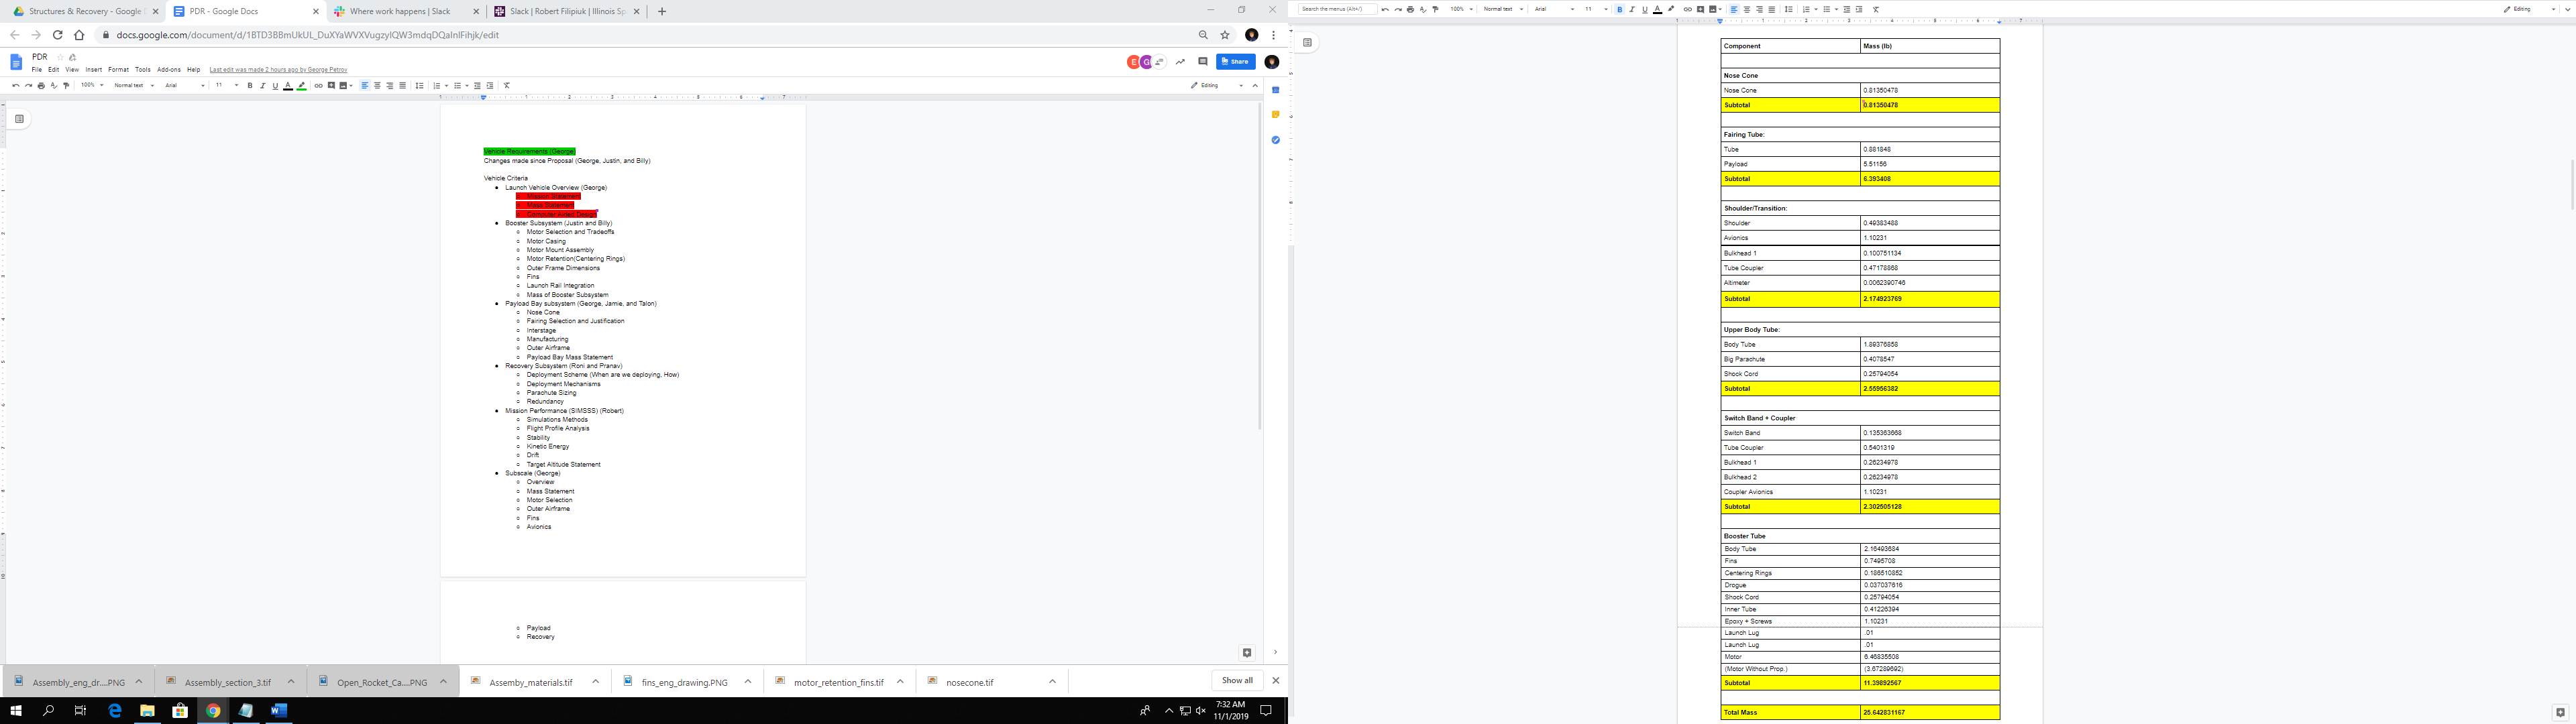
\includegraphics[width = 15cm, height = 20cm]{Masses.png}
    \caption{Predicted in-plane drift for various wind speeds and launch angles (all under spherical Earth approximation condition)}
    \label{fig:my_label}
\end{figure}

    \subsection{Mission Statement}
The rocket will ascend to a predefined altitude and return to the ground under parachutes. During descent, a drone will be deployed that is capable of detaching and flying to a target area to retrieve samples. The entirety of the mission will be conducted in accordance with all rules set forth by NASA in the 2020 NASA Student Launch Handbook.
   
    \subsection{Test Plan}
    \FloatBarrier
    \begin{figure}[h]
    \centering
    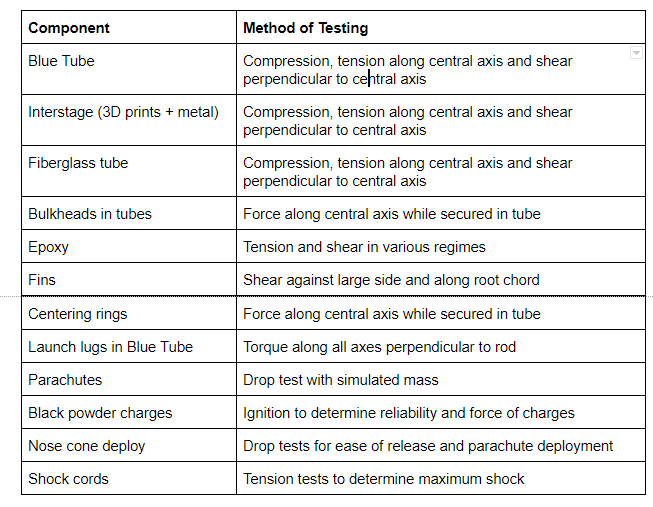
\includegraphics[width = 15cm, height = 20cm]{testplan.png}
    \caption{Predicted in-plane drift for various wind speeds and launch angles (all under spherical Earth approximation condition)}
    \label{fig:my_label}
\end{figure}

    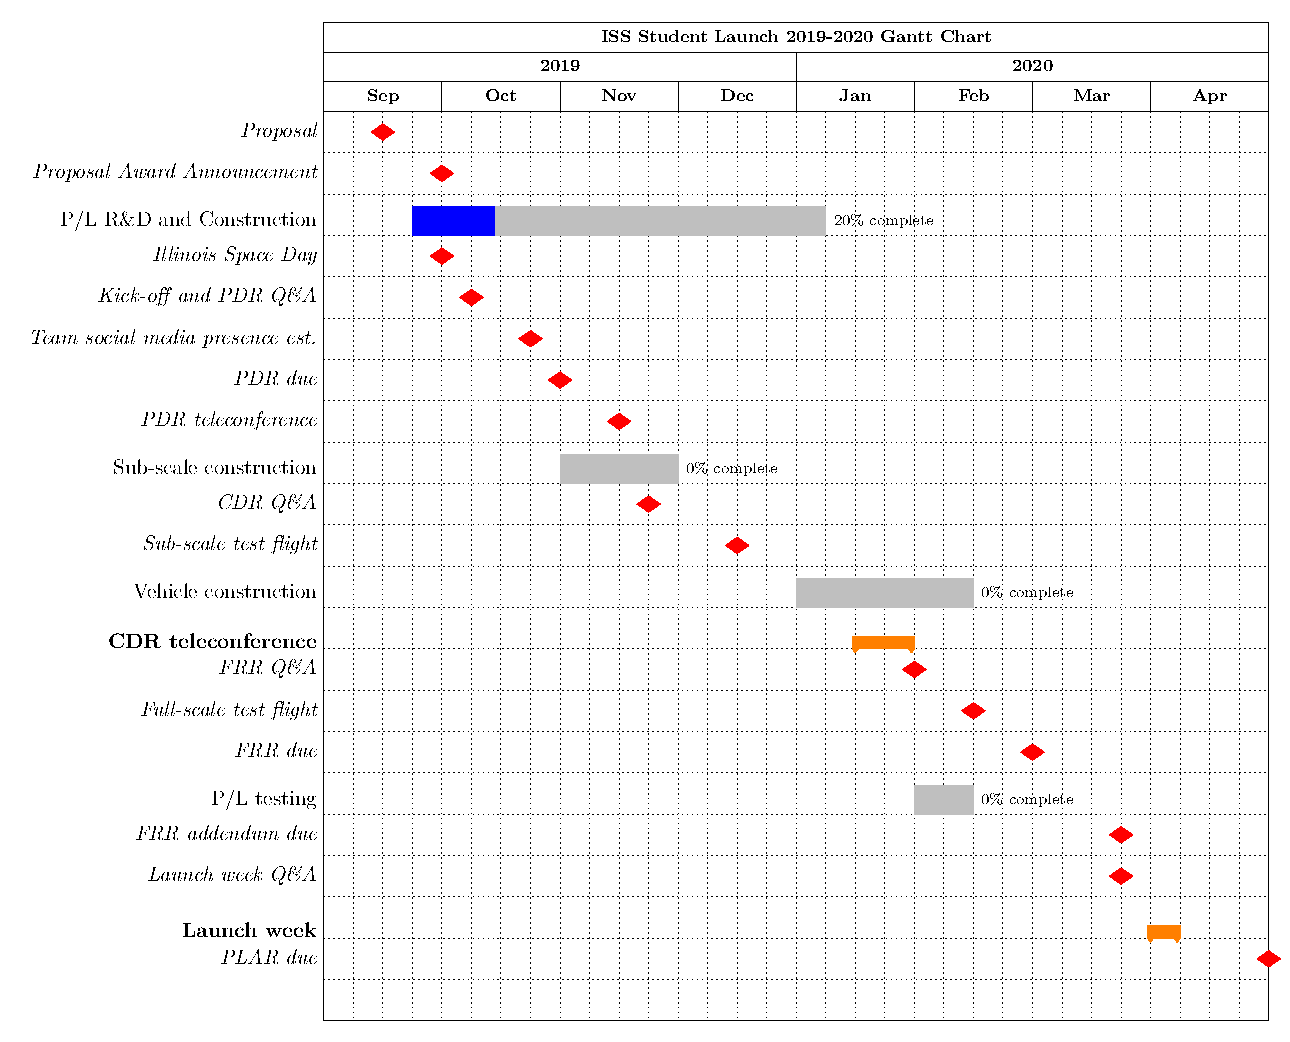
\includegraphics[width = 15cm, height = 10cm]{img/GanttChart.pdf}

\section{Booster Subsystem}
The booster subsystem is the lowest portion of the launch vehicle. It is primarily responsible for producing and properly containing the thrust of the rocket. The fins provide stability for the vehicle, ensuring a nominal trajectory. This subsystem also includes structural components that are necessary for safety and aerodynamics.

The main components of the booster subsystem are the motor, motor casing, motor mount, centering rings, outer airframe, and fins. Thrust is produced by the motor, while the motor casing, motor mounts, and centering rings are used to ensure the motor will maintain the correct orientation. The centering rings are mounted to the outer airframe and are arranged in such a way to direct the thrust vector through the vehicle’s center of mass.

The fins are an aerodynamic structure which collectively ensure stability and passive control for the launch vehicle. The overall subsystem is constructed to make sure that the rocket exits the launch rail with the desired velocity and stability and reaches the intended final altitude. A CAD model of the booster section is shown in [FIGURE HERE].

    \subsection{Motor Selection}
For the 2019-2020 Student launch competition, the team has chosen to use the AeroTech K780R-P motor. This motor satisfies all competition requirements since it keeps the target apogee within 3,500 feet and 5,500 feet above ground level, expels ammonium perchlorate composite propellant (APCP) during launch, has an impulse below the 5,120 Newton-Second limit, accelerates the launch vehicle beyond 52 feet per second upon exiting the rail, does not expel titanium sponges, is not a hybrid motor, is not clustered, and will not propel the launch vehicle above Mach 1 based on simulations. The motor is also able to be ignited using a 12-volt firing system and does not utilize any forward firing motors. According to updated OpenRocket simulations and the characteristics of the selected motor, the vehicle’s thrust-to-weight ratio is 8.5:1. Thrust-to-weight ratios greater than 5 are typically considered safe for high-powered rockets.

<<<<<<< HEAD
Performance specifications referred to in the table below and a thrust curve diagram for the K780R-P motor were found at thrustcurve.org. The motor reaches a maximum thrust of 216.9 pounds-force in about 1.15 seconds. The motor provides an average thrust of 175.4 pounds-force with a total burn time of 3.0 seconds.

\begin{table}[]
    {\footnotesize
    \caption{Motor Comparisons}
    \centering
    \begin{tabularx}{\linewidth}{XXXX}
    \toprule
    & AeroTech K780R & AeroTech K1000T & AMW K605RR \\ \midrule
    Diameter (in.) & 2.95 & 2.95 & 2.95 \\
    Length (in.) & 15.6 & 15.1 & 14.5 \\
    Total Weight (lb) & 6.468 & 5.736 & 6.104 \\
    Propellant Weight (lb) & 2.795 & 2.721 & 2.714 \\
    Average Thrust (lbf) & 175.4 & 239.6 & 136.0 \\
    Max. Thrust (lbf) & 216.9 & 376.3 & 165.8 \\
    Total Impulse (lbf-s) & 533.0 & 564.6 & 541.8 \\
    Burn Time (s) & 3.0 & 2.4 & 4.0 \\
    \bottomrule
    \end{tabularx}
    }
\end{table}
=======
Performance specifications [TABLE BELOW] and a thrust curve diagram [FIGURE BELOW] for the K780R-P motor were found at thrustcurve.org. The motor reaches a maximum thrust of 216.9 pounds-force in about 1.15 seconds. The motor provides an average thrust of 175.4 pounds-force with a total burn time of 3.0 seconds.
>>>>>>> f6ce28563d0bacd22907ad93059b1af2711fe643

In summary, the AeroTech K780R-P motor was chosen because it satisfies all necessary requirements stated within the guidelines provided for the Student Launch Competition. Other motors such as the Aerotech K1000T-P and Animal Motor Works K605RR were considered in the final decision, but it was determined that Aerotech was the favorable brand due to Illinois Space Society’s previous success with them, and the K1000T-P proved to provide too much impulse and caused the apogee to exceed competition guidelines with the final design of the rocket. Additionally, when compared to the K1000T-P, the K780R-P has lower acceleration over a slightly longer burn time, meaning structural loads on the rocket and payload are reduced.

    \subsection{Motor Casing}
The Aerotech 75/2560 motor casing will be used to house the K780R-P motor. It is the casing associated with this motor. It is made of aluminum, allowing it to withstand the high temperatures and forces created by the motor during launch. In addition, the top of the casing will serve as the lower attachment point for the drogue parachute. The length of the case is 15.577 inches with a diameter of 3.0 inches.


    \subsection{Motor Mount Assembly}
The motor mount assembly will consist of the motor mount tube, centering rings, and fins. The purpose of the motor mount is to keep the motor and motor casing in a stable position during flight. The motor mount tube will be constructed from a 15-inch length of Blue Tube with an outer diameter large enough to accomodate the motor casing. This tube, held in place by three fiberglass centering rings, will house the motor and motor casing.

Fiberglass was chosen for the centering rings as it is a strong material that will reduce the movement of the motor as much as possible without threat of deformation. These centering rings will have a thickness of 0.125 inches, and each will be epoxied onto the outside of the motor mount tube. The motor mount assembly also provides a rigid mount point for the fins. The three fiberglass fins will have fin tabs with a depth of 0.3 inches and a length of 5.2 inches beginning 1.2 inches from the bottom of the fin. This will allow them to be epoxied between the two lower centering ring prior to the insertion of the entire assembly into the lower airframe. An engineering drawing of the fin design can be seen in [FIGURE HERE]


    \subsection{Motor Retention}
A 2.95-inch Aero Pack motor retainer will be utilized. It is an aluminum part designed to keep the motor securely within the rocket during flight, as well as allow for quick and simple loading and unloading of the motor. The retainer will be screwed into the lower centering ring of the booster tube. Locknuts will be used on the opposite side of the screws holding in the retainer, ensuring that the connection will not be compromised in the event of high vibrations during flight. Though the screws are meant to allow reusability, the retainer will additionally be epoxied to the centering ring to provide added assurance that it will not come apart under any conditions. This mounting mechanism is threaded and has a matching cap that can be screwed on over the motor, thereby retaining it.

    \subsection{Outer Frame Dimensions}
In selecting a material for the outer airframe, the team considered three options: Blue Tube, fiberglass, and carbon fiber. Unanimously, the team voted on Blue Tube for the body tube and booster tube sections because of its low cost and its lower density, contributing less mass to the vehicle compared to fiberglass and carbon fiber. This low-cost, low-density justification is solely for these body tubes; fiberglass was chosen for the nose cone, fairing tube, and fairing because of the necessity for added strength in those sections. The team has had great success using Blue Tube for past projects. The launch vehicle’s fairing is expanded from the body tubes to ensure the ability to fit the payload. The primary booster tube has an outer diameter of 4 inches, while the fairing increases the diameter to 6 inches towards the top of the vehicle. The thicknesses of the booster tube, switch band, and body tube are all 0.118 inches. The thickness of the fairing, fairing body tube, and nose cone is 0.079 inches. This difference in material thickness is derived from the choice of material for each component of the launch vehicle. The components with thicknesses of 0.118 inches are comprised of Blue Tube, while the sections with thicknesses of 0.079 inches are fiberglass. A CAD model shows these materials in [FIGURE HERE]


    \subsection{Fins}
To ensure that the rocket is stable and maintains its intended flight path, three fins will be attached to the body tube with a radially symmetric separation of 120 degrees. Following a simulation using FinSim software, the decision was made to have the fin thickness be 0.125 inches because it provides high tensile strength that can withstand any possible aero-elastic forces while not being overly thick and diminishing the aerodynamic characteristics of the vehicle. 


    \subsection{Launch Rail Integration}
The purpose of integrating rail buttons is to ensure that the rocket is guided during launch until a sufficient velocity is attained at which the fins will stabilize the rocket. The incorporation of a mechanism to help guide the vehicle upon launch was difficult because of the choice to use a larger diameter fairing. In an effort to limit excess aerodynamic stress, it was decided that launch lugs will be attached to a threaded metal rod that is drilled into the body and booster tubes, and then attached by a nut and washer on the inside to ensure a secure mounting configuration. The cylindrical shape of the attaching rod will naturally have a lower drag coefficient than most other geometries, especially for off-trajectory winds.


\section{Payload Bay Subsystem}

    \subsection{Nose Cone}
    The nose cone design has changed significantly since the proposal. The overall shape has changed from an elliptical shape to tangent ogive shape. This came down to the manufacturing procedure that the team decided to take. Previously, the team was investigating the feasibility of manufacturing the nose cone in-house. This process would have involved creating an entire manufacturing rig, which would not have been within internal time constraints given the need to conduct extensive tests. The club has no prior experience in manufacturing fiberglass components of a rocket. This would take a lot of time and would be very difficult in the tight time frame. 

As a result, the nose cone will be bought commercially off the shelf. The produced size chosen has a 1 to 3 ratio of base diameter to length. This differed from an earlier plan to utilize a 2 to 3 ratio tangent ogive that would have been manufactured in-house. This change in ratio led to an increase in length of the nose cone.

The shape of the nose cone was changed from elliptical to tangent ogive because this shape is more aerodynamically efficient. The structural forces exerted on the nose cone will be considerably reduced with this shape. Since this is the area of the rocket that will experience the highest aerodynamic load, it is important to minimize forces to prevent overstressing the materials of the launch vehicle.

Other areas such as the body tube and booster tube have changed slightly. This is due to the evaluation of how much space each internal component will take up.

With the change in sizing of the outer airframe of the launch vehicle, the fins are crucial in keeping the stability above the required 2.0 cal. Due to this the size of the fins grew in size to keep the stability requirement.  


    \subsection{Fairing Selection and Justification}
 The integration of a fairing was ultimately decided because of the desire to minimize wasted space. In previous years, Illinois Space Society did not focus on maximizing the dimensions of the launch vehicle, but it was determined that it would greatly help reduce the cost of the launch vehicle as budgeting has been an issue in past years. The selected fairing size is 6 inches in diameter, extending via an interstage from a 4-inch body tube. The diameter of the body tube allows the motor to fit within it and provides adequate space for the parachutes, shock cords, and avionics. The fairing is wider to properly accommodate the team’s expected payload dimensions. A 4-inch diameter fairing would have been insufficient.


    \subsection{Interstage}
The interstage connecting the upper body tube and straight fairing tube will be a 3D printed cone that transitions from 4 inches at the base to 6 inches at the top. This diameter transition occurs over a length of 6 inches, thereby satisfying the requirement that each coupler/airframe element be longer than the width of the rocket. A bulkhead will be placed above the interstage in the fairing to aid in securing the segments together. The 3D print will be reinforced with vertical metal plates, each separated by 90 degrees, will then be placed inside the interstage. The plates will maintain the shape and help distribute the forces that may arise in this section during flight. The print and accompanying metal plates will be secured to the rocket using epoxy. A CAD model of this can be seen in [FIGURE HERE].

The nose cone is a pivotal component for any rocket. It reduces drag and shields the payload and other instruments from adverse ascent conditions. The team has chosen to use a 6-inch fiberglass ogive nose cone. When compared to various other nosecones, the fiberglass ogive was found to best meet the team’s needs. With regard to material, fiberglass offers the ideal compromise of being light, strong, and easy to work with.

At first, the team investigated manufacturing the nose cone using resin and molding techniques, but with time constraints and a lack of experience, it was decided that purchasing a nose cone would be significantly more efficient and likely much safer. Members of the team have worked with commercially purchased fiberglass in the past, so therein exists a better understanding of the risks associated with it. Fiberglass resin molding would introduce new risks in a process that is new to the team, which has been deemed undesirable. A CAD model of the current nose cone can be seen in [FIGURE HERE].



    \subsection{Manufacturing}
    Initially, the team planned to manufacture the nose cone and interstage in-house. Manufacturing in-house would provide a learning experience for the Illinois Space Society as the society has never developed these parts before. In order to manufacture, the team would need to design a system which would allow for molding. The preliminary plan for doing this was as follows. Foam would be cut to the desired design using a current flowing through a wire, giving the exact shape of the nose cone and interstage. After this, layers of fiberglass resin would be added on top of the cut foam to form to the desired shape. The fiberglass would then be cured and hardened. Due to the team having no prior experience with in-house manufacturing and the amount of time this process would require, the team decided commercially buying a nose cone will save both time, effort, and energy that could be devoted to different aspects of the rocket.
    
    \begin{table}[]
    \label{vertical unfolding arms}
    {\footnotesize
    \caption{Risk Matrix for Structure}
    \centering
    \begin{tabularx}{\linewidth}{XXXlXl}
    \toprule
    \textbf{Risk}                                            & \textbf{Cause}                                                                                                                 & \textbf{Impact}                                                                                                                           & \textbf{RBM}  & \textbf{Mitigation}                                                                                                                                                                                     & \textbf{RWM} \\ \midrule
    3D printed interstage support strain & Forces experienced during launch procedures & Launch Vehicle Interstage may lose adhesion or crack under stress & \cellcolor{orange!25} 1D & The 3D print infill will be increased and will extra attachment point for reinforcement materials & \cellcolor{green!25} 1E \\
    Launch lugs apply harmful torque to booster/body tube & Small attachment area at the tube & Tube would deform slightly at location of launch lug & \cellcolor{orange!25} 3C & The attachment area of the launch lug will be increased in order for torque to be evenly distributed & \cellcolor{green!25} 3E \\
    Drogue fails to deploy & Ejection charge fails to fire & Launch Vehicle lands at a dangerous velocity & \cellcolor{red!25} 1C & Test ejection charge system for continuity before hand and use redundant charges and altimeters & \cellcolor{green!25} 1E \\
    Main parachute fails to deploy & Defect in parachute release & Damage to booster and body tube of launch vehicle & \cellcolor{red!25} 1C & Test ejection charge system for continuity before hand and use redundant charges and altimeters & \cellcolor{green!25} 1E \\ \midrule
    Fins shear off & Excessive aerodynamic forces during flight & Rocket loses stability & \cellcolor{orange!25} 1D & Fins will be attached inside to body tube using laminating epoxy to ensure resistance to aerodynamic shear forces & \cellcolor{orange!25} 1D \\
    Nose cone separation fails & CO2 canister does not fire & Payload trapped in descending rocket & \cellcolor{orange!25} 2D & Ground testing and calculations for CO2 pressure and operation & \cellcolor{green!25} 2E \\
    Nose cone parachute deployment fails & Parachute release either opens too early or not at all & Nose cone drifts too far or goes ballistic & \cellcolor{green!25} 3D & Pre-flight procedures include chute release as parachute packing procedure & \cellcolor{green!25} 3E \\
    Motor retainer fails & Poorly secured & Motor falls out the bottom of the rocket & \cellcolor{red!25} 1C & Secure motor retainer to lower centering ring using epoxy while also ensuring to retainer cap is secure before launch & \cellcolor{green!25} 1E \\
    Motor ignition fails & Igniter is not securely placed & Launch vehicle fail to launch & \cellcolor{green!25} 4B & Ensure igniter is placed as far up to motor as possible and review launch sequence beforehand & 4D \\
    Launch Vehicle drifts excessively far into hazardous terrain & Main parachute deployment at apogee & Vehicle components are unrecoverable or require excessive time to locate & \cellcolor{orange!25} 2C & Model the vehicle’s flight characteristics and size parachutes appropriately to minimize drift distance. & \cellcolor{orange!25} 2D \\
    Vehicle spins excessively during launch & Improperly aligned fins & Possible damage to sensitive internal components & \cellcolor{red!25} 2B & Be sure that fins are assembled adequately and use fin jig during construction to ensure vertical alignment & \cellcolor{green!25} 2E \\
    Motor ignites prematurely & Igniter triggers prematurely and fuel grain is exposed to open flame & Vehicle launches unexpectedly & \cellcolor{red!25} 2B & Keep open flames away from launch vehicle at all times during setup and arm igniter immediately before launch & \cellcolor{green!25} 2E\\
    \bottomrule
    \end{tabularx}
    }
\end{table}

Commercially buying a nose cone will allow more time for research in areas besides manufacturing. With deadlines such as the upcoming subscale launch in December, buying the nose cone will allow more time to complete the launch vehicle. The nose cone, which will be purchased from Madcow Rocketry, will be structurally sound as it is manufactured by professionals. The Illinois Space Society views the proven integrity of a commercial nose cone as a way to minimize risk because of the team’s lack of experience in nose cone manufacturing.
 
The launch vehicle will be comprised mostly of parts that were commercially bought rather than manufactured. This allows more time and effort to be put into the construction and testing of the rocket. Since the team members have a lack of experience with fiberglass molds, structural integrity was a major risk factor. Although it would be beneficial to gain experience, the risks that go along with such a feat do not outweigh the benefits in this scenario. Buying the nose cone commercially would also be more cost effective as the team does not know how many attempts it would take to produce a nose cone of sufficient specifications to survive flight, making it unclear how much resin would be used per attempt. 
